\documentclass{article}
\newenvironment{standalone}{\begin{preview}}{\end{preview}}
\usepackage{../includes}

\begin{document}
\begin{standalone}

  \section{Resultados}

  Una vez que la aplicación en Unity está lista, se compila y ejecuta en el teléfono \textit{File >\ Build and Run}.
  Se asegura que la Raspberry Pi esté ejecutando el script de servidor y que los códigos QR estén colocados adecuadamente en el sitio a navegar.

  Al iniciar la aplicación, se pide en primer lugar descargar los datos de navegación.
  La \cref{fig:captura_1} muestra la selección del dispositivo bluetooth para la descarga de datos de navegación.
  En la \cref{fig:captura_2} se ve el mensaje recibido con dichos datos.
  En la \cref{fig:captura_3} el usuario selecciona el destino.
  Ya se puede ver el minimapa en la esquina inferior izquierda.
  Las \cref{fig:captura_4,fig:captura_5} muestran la asistencia a la navegación tanto en el minimapa como con objetos de realidad aumentada.

  \begin{figure}[ht!]
    \centering
    \begin{subfigure}[b]{0.19\textwidth}
      \centering
      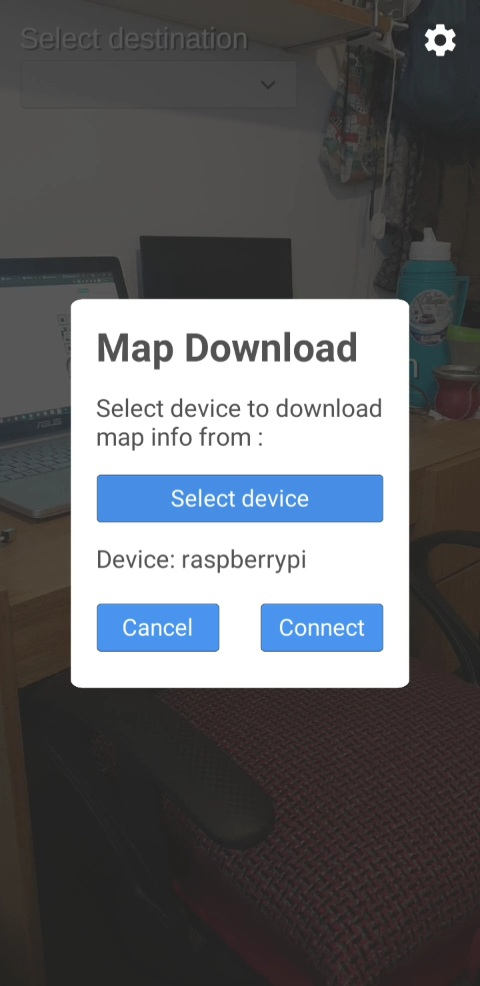
\includegraphics[width=\textwidth]{captura_1}
      \caption{}
      \label{fig:captura_1}
    \end{subfigure}
    \hfill
    \begin{subfigure}[b]{0.19\textwidth}
      \centering
      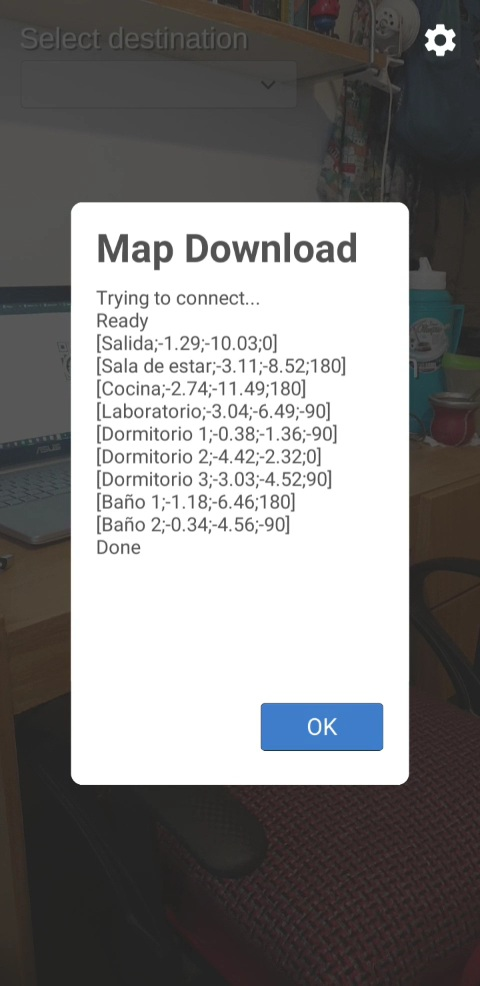
\includegraphics[width=\textwidth]{captura_2}
      \caption{}
      \label{fig:captura_2}
    \end{subfigure}
    \hfill
    \begin{subfigure}[b]{0.19\textwidth}
      \centering
      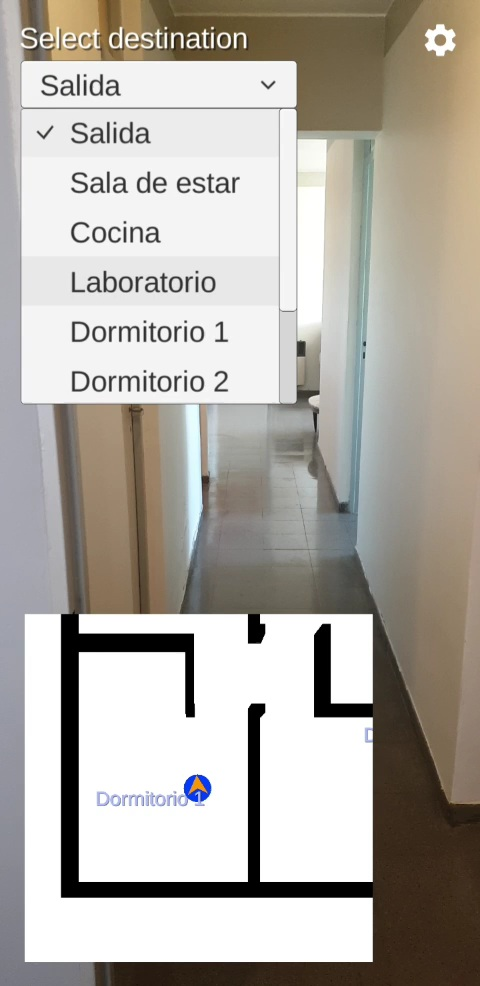
\includegraphics[width=\textwidth]{captura_3}
      \caption{}
      \label{fig:captura_3}
    \end{subfigure}
    \hfill
    \begin{subfigure}[b]{0.19\textwidth}
      \centering
      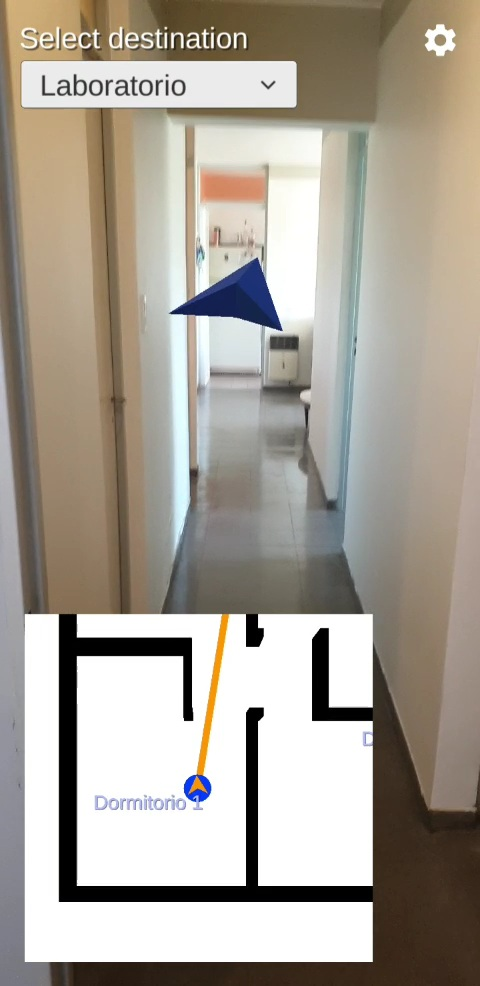
\includegraphics[width=\textwidth]{captura_4}
      \caption{}
      \label{fig:captura_4}
    \end{subfigure}
    \hfill
    \begin{subfigure}[b]{0.19\textwidth}
      \centering
      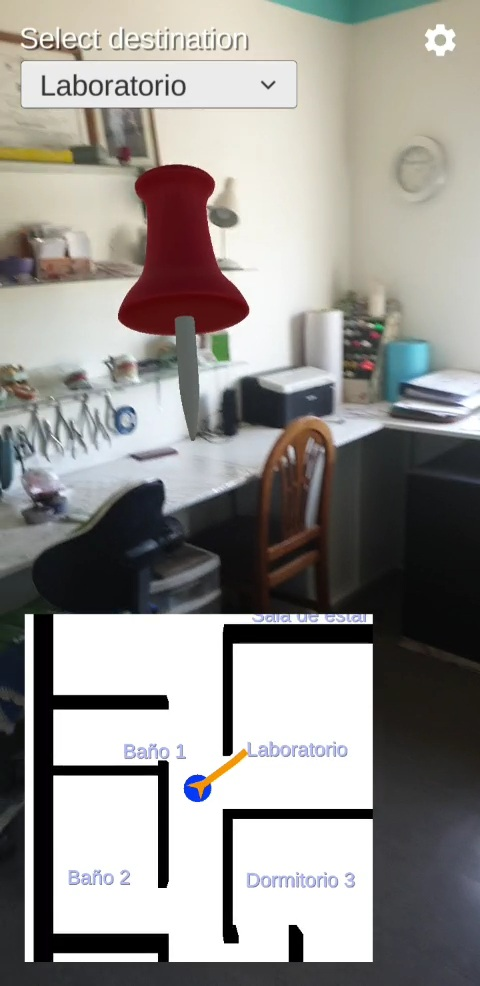
\includegraphics[width=\textwidth]{captura_5}
      \caption{}
      \label{fig:captura_5}
    \end{subfigure}
    \hfill

    \caption{Captura de la aplicación en ejecución.}
    \label{fig:capturas}
  \end{figure}

  Puede comprobarse que, de manera general, la aplicación funciona correctamente pero, como se dijo anteriormente, el seguimiento de movimiento tiene errores acumulativos.
  Y estos se agravan cuando hay poca iluminación, cuando se realizan movimientos bruscos y cuando hay pocos puntos reconocibles, por ejemplo, cuando se apunta a la pared de un pasillo.

  También se comprobó el efecto de activar o desactivar el componente \textit{NavMeshAgent} del objeto usuario.
  Cuando está desactivado, el usuario puede atravesar paredes debido a los errores inherentes del seguimiento de movimiento.
  Esto produce indicaciones de navegación erróneas.
  Cuando está habilitado, el usuario no puede atravesar paredes, pero puede quedar atrapado en una habitación equivocada y produciendo también indicaciones falsas pero más consistentes.

  % Bajo estas circunstancias, la navegación puede fallar, pero se soluciona rápidamente escaneando un nuevo código QR para la relocalización.
  Para todas estas situaciones en las que la navegación puede fallar, se soluciona rápidamente con recalibración escaneando un nuevo código QR para la relocalización del usuario.

\end{standalone}
\end{document}
